\documentclass[../main.tex]{subfiles}
\begin{document}
\section{马尔可夫决策过程与强化学习}\label{sec:mdp-rl}
\subsection{马尔可夫决策过程（MDP）}\label{sec:mdp}
\begin{enumerate}
    \item \textbf{马尔可夫性质：}在某一任务中，如果Agent从环境中得到的下一状态仅依赖于当前状态，而不考虑历史状态，即
    $$P\left\lbrack  {{S}_{t + 1} \mid  {S}_{t}}\right\rbrack   = P\left\lbrack  {{S}_{t + 1} \mid  {S}_{1},\ldots ,{S}_{t}}\right\rbrack$$
    \item \textbf{马尔可夫过程(Markov Process, MP)：}由二元组(S,S)中的 $\left( {{S}_{t},{S}_{t + 1}}\right)$ 组成的马尔可夫链,该链中的所有状态都满足马尔可夫性质。
    \item \textbf{马尔可夫奖赏过程(Markov Reward Process, MRP)：}由三元组(S,P,R)组成的马尔可夫过程。根据概率,状态自发地进行转移, 其状态转移概率 $P$ 与动作无关, 记为:
    $$P\left\lbrack  {{S}_{t + 1} = {s}^{\prime } \mid  {S}_{t} = s}\right\rbrack$$
    \item \textbf{马尔可夫决策过程(Markov Decision Process,MDP)：}由四元组(S,A,P,R)组成的马尔可夫过程,状态依靠动作进行转移。马尔可夫决策过程分为:
    \begin{itemize}
        \item 有穷马尔可夫决策过程；
        \item 无穷马尔可夫决策过程；
    \end{itemize}
    \item \textbf{MDP四个基本元素：}
    \begin{enumerate}
        \item \textbf{状态（State）或观测值（Observation）：}
        马尔可夫决策过程中的状态空间通常记为 $S$
        \begin{itemize}
            \item $S$：表示不包含终止状态的状态空间；
            \item $S^+$：表示包含终止状态的状态空间；
            \item $s$：表示状态空间中的某一个状态，通常用向量表示；
            \item 状态可分为\textbf{离散状态}和\textbf{连续状态}两类。
        \end{itemize}

        \item \textbf{动作（Action）：}
        动作空间通常记为 $A$，表示 Agent 在环境中可采取的动作集合。
        \begin{itemize}
            \item $A$：表示动作空间；
            \item $A(s)$：表示在状态 $s$ 下可执行的动作空间；
            \item $a$：表示动作空间中的某一个动作；
            \item 动作通常也可分为\textbf{离散动作}和\textbf{连续动作}两类。
        \end{itemize}

        \item \textbf{状态转移（State Transition）：}
        状态转移概率通常记为 $p$，表示在当前状态 $s$ 下执行动作 $a$ 后转移到下一状态 $s'$ 的概率。
        \begin{itemize}
            \item 联合写法：
            $$
            p(s',r\mid s,a)=P\left[ S_{t+1}=s',R_{t+1}=r \mid S_t=s,A_t=a\right],\qquad \sum_{s'}\sum_r p(s',r\mid s,a)=1
            $$
            \item 只考虑状态转移时可写为：
            $$
            p(s'\mid s,a)=P\left[ S_{t+1}=s' \mid S_t=s,A_t=a\right],\qquad \sum_{s'} p(s'\mid s,a)=1
            $$
            \item 若某一转移结果是确定的，则称为\textbf{确定环境}；
            \item 若同一状态动作对可能对应多个不同结果，则称为\textbf{随机环境}。
        \end{itemize}

        \item \textbf{奖赏（Reward）：}
        奖赏空间通常记为 $R$，表示 Agent 在环境中采取动作后所获得的反馈。
        \begin{itemize}
            \item $R$：表示奖赏空间；
            \item $r(s,a,s')$：表示 Agent 在状态 $s$ 下执行动作 $a$ 并转移到状态 $s'$ 时获得的期望奖赏；
            \item 奖赏可分为\textbf{离散奖赏}和\textbf{连续奖赏}两类。
        \end{itemize}
        奖赏函数可写为：
        $$
        r(s,a,s')=E\left[ R_{t+1}\mid S_t=s,A_t=a,S_{t+1}=s'\right]
        =\sum_r r\frac{p(s',r\mid s,a)}{p(s'\mid s,a)}
        $$
        也可写为：
        $$
        r(s,a)=E\left[ R_{t+1}\mid S_t=s,A_t=a\right]
        =\sum_r\sum_{s'} r\,p(s',r\mid s,a)
        $$
        对于奖赏，可以从两个角度理解：
        \begin{itemize}
            \item 先获得奖赏，再进入下一状态：此时奖赏 $R_{t+1}$ 与当前状态 $S_t$ 和动作 $A_t$ 相关；
            \item 先进入下一状态，再获得奖赏：此时奖赏 $R_{t+1}$ 与当前状态 $S_t$、动作 $A_t$ 以及下一状态 $S_{t+1}$ 相关。
        \end{itemize}
        \textcolor{red}{下面这个题我觉得构建状态转移概率的时候那个“if”（当...时）写的不太好，似乎把很多非法状态，比如撞墙都算进去了，我觉得其实可以写的更好。
        }
        {\small\kaishu
        \item \textbf{常考：扫地机器人任务的MDP数学建模}\label{sweep_robot}
        \begin{enumerate}
            \item \textbf{题目条件：}
            考虑一个 $5\times 5$ 的网格环境，机器人需要在躲避障碍物的同时，到指定位置收集垃圾，并可到指定位置充电。其中：
            \begin{itemize}
                \item 充电位置为 $[1,1]$；
                \item 垃圾位置为 $[5,4]$；
                \item 障碍物位置为 $[3,3]$。
            \end{itemize}
        
            \item \textbf{状态空间 $S$：}
            将环境离散化为 $24$ 个状态（去掉障碍物 $[3,3]$），可表示为
            $$
            \begin{aligned}
            S=\{&[1,1],[2,1],[3,1],[4,1],[5,1],\\
                &[1,2],[2,2],[3,2],[4,2],[5,2],\\
                &[1,3],[2,3],[4,3],[5,3],\\
                &[1,4],[2,4],[3,4],[4,4],[5,4],\\
                &[1,5],[2,5],[3,5],[4,5],[5,5]\}
            \end{aligned}
            $$
            
            \item \textbf{动作空间 $A$：}
            机器人每一步可采取四个离散动作
            $$
            A=\{\text{上}:[0,1],\ \text{下}:[0,-1],\ \text{左}:[-1,0],\ \text{右}:[1,0]\}
            $$
        
            \item \textbf{确定环境下的四元组 $(S,A,P,R)$：}
            \begin{itemize}
                \item \textbf{条件：}动作执行后状态唯一确定；若到达垃圾点或充电点则停留在原状态；若动作会撞向障碍物，则保持原地不动。
                
                \item \textbf{状态转移函数 $P$：}
                记状态转移函数为
                $$
                f(s,a)=
                \begin{cases}
                s+a, & s\neq [1,1],\ s\neq [5,4],\ \text{且 } s+a\neq [3,3] \\
                s, & \text{其他}
                \end{cases}
                $$
                因而状态转移概率为
                $$
                p(s,a,s')=
                \begin{cases}
                1, & (s+a=s' \text{ 且 } s+a\neq [3,3]) \\
                   & \text{或 } ((s=[1,1]\ \text{或}\ s=[5,4]\ \text{或}\ s+a=[3,3]) \text{ 且 } s=s') \\
                0, & \text{其他}
                \end{cases}
                $$
                
                \item \textbf{奖赏函数 $R$：}
                根据题意：
                \begin{itemize}
                    \item 到达垃圾位置 $[5,4]$ 时，得到 $+3$ 的奖赏；
                    \item 到达充电位置 $[1,1]$ 时，得到 $+1$ 的奖赏；
                    \item 若动作会使机器人撞向障碍物 $[3,3]$，则保持原地不动，并得到 $-10$ 的奖赏；
                    \item 其他情况奖赏为 $0$。
                \end{itemize}
                因此可写为
                $$
                r(s,a)=
                \begin{cases}
                +3, & \text{如果 } s\neq [5,4] \text{ 且 } s+a=[5,4] \\
                +1, & \text{如果 } s\neq [1,1] \text{ 且 } s+a=[1,1] \\
                -10, & \text{如果 } s+a=[3,3] \\
                0, & \text{其他}
                \end{cases}
                $$
            \end{itemize}
        
            \item \textbf{随机环境下的四元组 $(S,A,P,R)$：}
            \begin{itemize}
                \item \textbf{条件：}状态空间和动作空间与确定环境相同，但状态转移不再确定。若机器人尝试向某一方向移动，则：
                \begin{itemize}
                    \item 成功移动到目标方向的概率为 $0.80$；
                    \item 保持原地不动的概率为 $0.15$；
                    \item 移动到相反方向的概率为 $0.05$。
                \end{itemize}
                
                \item \textbf{状态转移函数 $P$：}
                因而状态转移概率可写为
                $$
                p(s,a,s')=
                \begin{cases}
                0.80, & \text{如果 } s+a=s' \text{ 且 } s\neq s' \\
                0.15, & \text{如果 } s=s' \text{ 且 } s\neq [1,1] \text{ 且 } s\neq [5,4] \\
                0.05, & \text{如果 } s-a=s' \text{ 且 } s\neq s' \\
                0, & \text{其他}
                \end{cases}
                $$
                
                \item \textbf{奖赏函数 $R$：}
                在随机环境下，奖赏不仅与 $(s,a)$ 有关，还与下一状态 $s'$ 有关。根据题意：
                \begin{itemize}
                    \item 若下一状态到达垃圾位置 $[5,4]$，则得到 $+3$；
                    \item 若下一状态到达充电位置 $[1,1]$，则得到 $+1$；
                    \item 若机器人朝障碍物方向运动并因此保持原地不动，则得到 $-10$；
                    \item 其他情况奖赏为 $0$。
                \end{itemize}
                因此可写为
                $$
                r(s,a,s')=
                \begin{cases}
                +3, & \text{如果 } s\neq [5,4] \text{ 且 } s'=[5,4] \\
                +1, & \text{如果 } s\neq [1,1] \text{ 且 } s'=[1,1] \\
                -10, & \text{如果 } s+a=[3,3] \text{ 且 } s=s' \\
                0, & \text{其他}
                \end{cases}
                $$
            \end{itemize}
        \end{enumerate}
        }
    \end{enumerate}
\end{enumerate}

\begin{figure}[H]
    \centering
    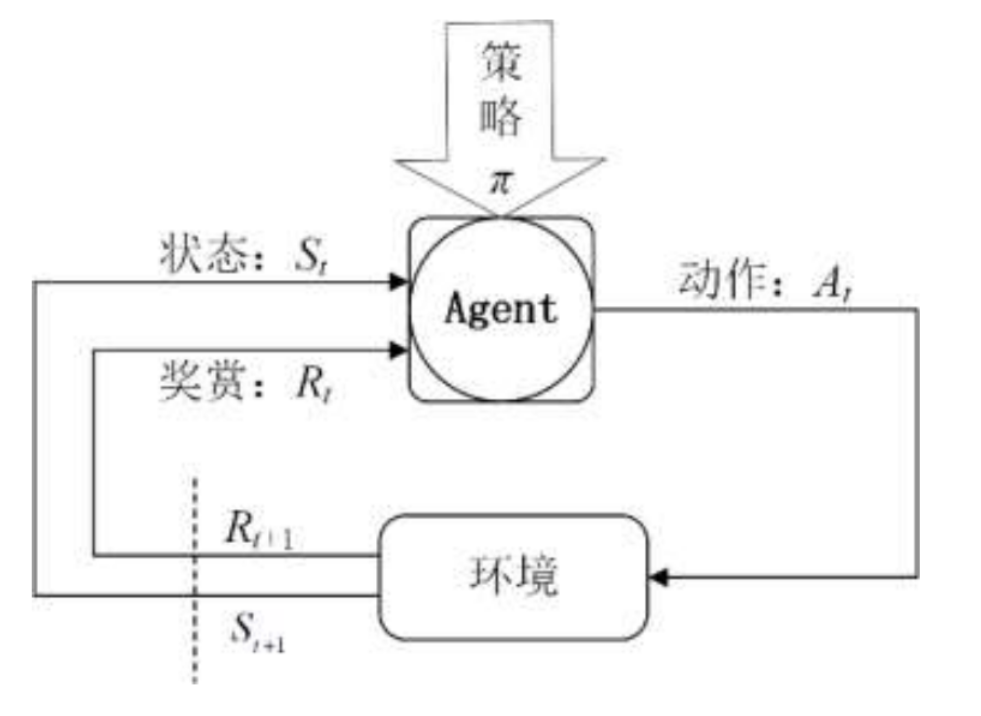
\includegraphics[width=0.55\linewidth]{images/mdp.png}
    \caption{基于MDP强化学习的基本框架}
    \label{fig:placeholder}
\end{figure}
\subsection{强化学习}\label{sec:reinforcement-learning}
\begin{enumerate}
    \item \textbf{含义：}从环境状态到行为映射的学习，以使系统行为从环境中获得的累积奖赏（reward）最大；三类机器学习方法之一（监督学习、无监督学习、强化学习）。
    
    \item \textbf{特点：}
    \begin{itemize}
        \item 没有监督数据，只有 reward；
        \item 反馈有延时，不是立即返回；
        \item 数据是序列化的，数据与数据之间是有关联的，而不是 i.i.d\footnote{independent and identically distributed，独立同分布} 的；
        \item Agent 执行的动作会影响之后的数据。
    \end{itemize}
    
    \item \textbf{预测与控制：}
    \begin{itemize}
        \item \textbf{预测：}给定某个策略，估计该策略下每个状态或状态动作对的价值；
        \item \textbf{控制：}找到一个最优的策略；
        \item 在 RL 算法中，通常都是迭代地进行先预测，再控制的过程，直到收敛。
    \end{itemize}
    
    \item \textbf{拓展：}深度强化学习，是一种端到端（end-to-end）的感知与控制系统，具有很强的通用性。
    
    \item \textbf{学习方法分类：}
    \begin{enumerate}
        \item \textbf{按环境模型分类：}
        \begin{itemize}
            \item \textbf{基于模型（model-based）：}状态转移概率 $p$ 已知，能够通过建立完备的环境模型来模拟真实反馈。
            \begin{itemize}
                \item \textbf{相关算法：}动态规划法（DP）。
                \item \textbf{优点：}
                \begin{itemize}
                    \item 能够基于模拟经验数据直接模拟真实环境；
                    \item 具备推理能力，能够直接评估策略的优劣性；
                    \item 能够与监督学习算法相结合，来求解环境模型。
                \end{itemize}
                \item \textbf{缺点：}\footnote{第一次近似误差：环境模型没学准。第二次近似误差：在不够准确的模型上继续学值函数或策略，又学偏了。}
                \begin{itemize}
                    \item 第一次近似误差：基于真实经验对模型进行学习，得到的模型仅仅是 Agent 对环境的近似描述；
                    \item 第二次近似误差：基于模拟模型对值函数或策略进行学习时，存在学习误差。
                \end{itemize}
            \end{itemize}
            
            \item \textbf{无模型（model-free）：}状态转移概率 $p$ 未知，Agent 所处的环境模型是未知的。
            \begin{itemize}
                \item \textbf{特点：}不试图显式建立环境模型，而是根据与环境交互得到的反馈直接学习；
                \item \textbf{相关算法：}Q-learning、Sarsa、蒙特卡洛法、时序差分法、值函数近似、策略梯度法。
            \end{itemize}
        \end{itemize}
        
        \item \textbf{按更新方式分类：}
        \begin{itemize}
            \item \textbf{回合更新：}一个回合结束后再进行更新，即 episode by episode。
            \begin{itemize}
                \item \textbf{典型方法：}蒙特卡洛（MC）、REINFORCE。
            \end{itemize}
            
            \item \textbf{单步更新：}不需要等到回合结束，而是每一步都进行更新，即 step by step。
            \begin{itemize}
                \item \textbf{典型方法：}Q-learning、Sarsa、策略梯度法。
            \end{itemize}
        \end{itemize}
        
        \item \textbf{按求解方式分类：}
        \begin{itemize}
            \item \textbf{基于价值（value-based）：}目标是学习状态或状态动作对的价值，再根据价值选择动作；一般更适用于离散动作情形。
            \begin{itemize}
                \item \textbf{典型方法：}Q-learning、Sarsa。
            \end{itemize}
            
            \item \textbf{基于策略（policy-based）：}目标是直接学习策略，输出各动作的概率分布或直接输出动作；适用于连续动作情形。
            \begin{itemize}
                \item \textbf{典型方法：}策略梯度、AC。
            \end{itemize}
        \end{itemize}
        
        \item \textbf{按策略使用分类：}
        \begin{itemize}
            \item \textbf{同策略（on-policy）：}目标策略和行为策略相同。
            \begin{itemize}
                \item \textbf{典型方法：}Sarsa、Sarsa($0$)、TRPO。
            \end{itemize}
            
            \item \textbf{异策略（off-policy）：}目标策略和行为策略不同。
            \begin{itemize}
                \item \textbf{典型方法：}Q-learning、DQN、确定性策略梯度。
            \end{itemize}
            
            \item \textbf{区别：}更新 $Q$ 值\footnote{在状态 s 下采取动作 a 后，未来能够获得的期望累计回报}时，使用的是既定策略还是新的策略\footnote{同策略与异策略的区别，在于更新当前 $Q$ 值时，对未来部分采用哪一种假设。设智能体在状态 $s$ 下实际执行了动作 $a$，到达下一状态 $s'$。两类方法都会用这次真实交互得到的即时奖励 $r$ 来更新 $Q(s,a)$；区别在于，对后续回报的估计不同：同策略方法使用行为策略在 $s'$ 下实际或将要选择的动作来估计未来价值；异策略方法则不管行为策略下一步实际怎么选，而是假设后续按目标策略行动，并用目标策略对应的动作价值来估计未来回报。}
            \item \textbf{异策略的特点：}
            \begin{itemize}
                \item 可以从人类给出的示教样本或其他智能体给出的引导样本中学习；
                \item 可以重用由旧策略生成的经验；
                \item 可以在使用一个探索性策略的同时，学习一个确定性策略；
                \item 可以用一个策略进行采样，同时学习多个策略。
            \end{itemize}
        \end{itemize}
    \end{enumerate}
\end{enumerate}


\subsection{求解强化学习任务}\label{sec:rl-solving}
强化学习的目的就是：在MDP中搜索到最优策略。
\begin{enumerate}
    \item \textbf{策略：}策略表示状态到动作的映射，即在状态 $s$ 下采取动作 $a$ 的概率，记为
    $$
    \pi(a\mid s)=P(A_t=a\mid S_t=s)
    $$
    \begin{itemize}
        \item 按照输出形式，策略可分为：
        \begin{itemize}
            \item \textbf{确定策略：}在每个状态下只选择一个确定动作；
            $$a = \pi \left( s\right)$$
            \item \textbf{随机策略：}在每个状态下按某个概率分布选择动作。
            $$\pi \left( {a \mid  s}\right)  = P\left( {a \mid  s}\right)  = P\left( {{A}_{t} = a \mid  {\mathbf{S}}_{t} = s}\right)$$
        \end{itemize}
    
        \item 按照用途，策略可分为：
        \begin{itemize}
            \item \textbf{行为策略：}Agent 实际与环境交互并生成样本所使用的策略；
            \item \textbf{目标策略：}需要学习、评估或优化的策略。
        \end{itemize}
    \end{itemize}

    \item \textbf{强化学习任务的两种随机性:}
    \begin{itemize}
        \item \textbf{策略随机性：}人为设定的$\pi \left( {a \mid  s}\right) $
        \item \textbf{状态转移随机性：}人为设定的$p(s^{\prime},r\mid s,a)$
    \end{itemize}
    \item \textbf{MDP一个策略产生序列的方法：}
    \begin{enumerate}
        \item 从初始状态分布中产生一个初始状态 $S_i=S_0$；
        \item 根据策略 $\pi(a\mid S_i)$，给出采取的动作 $A_i$，并执行该动作 $A_i$；
        \item 根据奖赏函数和状态转移函数得到奖赏 $R_{i+1}$ 和下一个状态 $S_{i+1}$；
        \item 令 $S_i=S_{i+1}$；
        \item 不断重复第（2）步到第（4）步的过程，产生一个序列：
        $$
        S_0,A_0,R_1,S_1,A_1,R_2,S_2,A_2,R_3,S_3,\cdots
        $$
        \item 如果任务是回合式\footnote{episodic，ppt中机翻为“情节式”}的，序列将终止于状态 $S_{\text{goal}}$；如果任务是连续式的，序列将无穷延续。
    \end{enumerate}
    
    \item \textbf{奖赏与回报：}
    \begin{itemize}
        \item 定义马尔可夫决策过程的回报如下：
        $$
        G_t=R_{t+1}+R_{t+2}+\cdots+R_T
        $$
        \item 实际情况中，需要引入折扣率 $\gamma$，用于对未来奖赏赋予折扣，则回报定义如下：
        $$
        G_t=R_{t+1}+\gamma R_{t+2}+\gamma^2 R_{t+3}+\cdots,\qquad \gamma\in[0,1]
        $$
        \item 折扣回报还可写成递推形式：
        $$
        G_t=R_{t+1}+\gamma G_{t+1}
        $$
    \end{itemize}

    {\small\kaishu
    例题：设折扣率 $\gamma=0.2$，$T=4$，奖赏序列为
        $$
        R_1=2,\quad R_2=1,\quad R_3=5,\quad R_4=4
        $$
        计算各时刻的回报：$G_0,G_1,\cdots,G_4$。
        \begin{align*}
        G_4 &= 0 \\
        G_3 &= R_4+\gamma G_4 = 4+0.2\times 0 = 4 \\
        G_2 &= R_3+\gamma G_3 = 5+0.2\times 4 = 5.8 \\
        G_1 &= R_2+\gamma G_2 = 1+0.2\times 5.8 = 2.16 \\
        G_0 &= R_1+\gamma G_1 = 2+0.2\times 2.16 = 2.432
        \end{align*}
    }


    
    \item \textbf{值函数\footnote{说人话就是从当前状态出发，未来还能有多大长期收益}与贝尔曼方程\footnote{值函数是未知目标，贝尔曼方程是约束这些未知目标的方程}：}
    
    \textcolor{red}{感觉不太可能考这个吧？就算考把贝尔曼方程背下来就行，本质上就是跟着状态值函数更新图的Markov过程，纯粹就是高中条件概率题，别看符号多，其实很好理解}
    \begin{itemize}
        \item \textbf{状态值函数（state-value function）：}
    
        状态值函数 $v_{\pi}(s)$ 表示遵循策略 $\pi$ 时，状态 $s$ 的价值。可表示为：
        $$
        v_{\pi}(s)=\mathbb{E}_{\pi}(G_t\mid S_t=s)
        $$
    
        \item \textbf{动作值函数（action-value function）：}
    
        动作值函数 $q_{\pi}(s,a)$ 表示遵循策略 $\pi$ 时，在状态 $s$ 采取动作 $a$ 的价值。可表示为：
        $$
        q_{\pi}(s,a)=\mathbb{E}_{\pi}(G_t\mid S_t=s,A_t=a)
        $$
    
        \item \textbf{状态值函数的贝尔曼方程：}
    
        动作值函数是在状态值函数的基础上考虑了执行动作 $a$ 所产生的影响，于是可以构建值函数的递归关系：
        $$
        \begin{aligned}
        v_{\pi}(s)
        &=\mathbb{E}_{\pi}(G_t\mid S_t=s)\\
        &=\mathbb{E}_{\pi}(R_{t+1}+\gamma G_{t+1}\mid S_t=s)\\
        &=\sum_{a}\pi(a\mid s)\sum_{s',r}p(s',r\mid s,a)\Big[r+\gamma \mathbb{E}_{\pi}(G_{t+1}\mid S_{t+1}=s')\Big]\\
        &=\sum_{a}\pi(a\mid s)\sum_{s',r}p(s',r\mid s,a)\big[r+\gamma v_{\pi}(s')\big]
        \end{aligned}
        $$
    \begin{figure}[H]
        \centering
        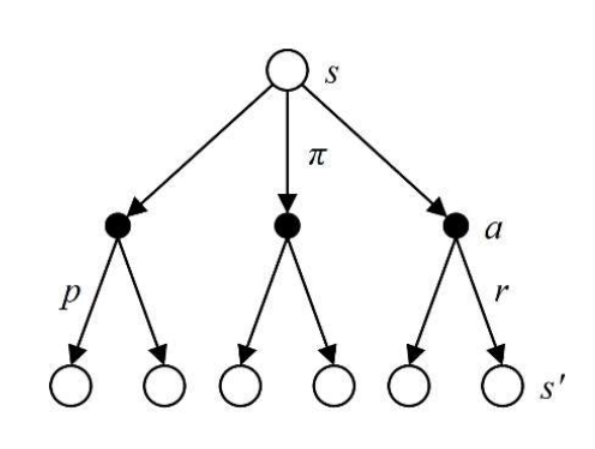
\includegraphics[width=0.45\linewidth]{images/rl.png}
        \caption{状态值函数更新图}
        \label{fig:placeholder}
    \end{figure}
        \item 根据状态值函数贝尔曼方程，可以构建状态值函数更新图。空心圆表示状态，实心圆表示动作。由图可知，状态值函数与动作值函数满足如下关系式：
        $$
        v_{\pi}(s)=\sum_{a}\pi(a\mid s)q_{\pi}(s,a)
        $$
    
        \item \textbf{动作值函数的贝尔曼方程：}
    
        与状态值函数的贝尔曼方程推导方式类似，同理可以得到动作值函数的贝尔曼方程：
        $$
        \begin{aligned}
        q_{\pi}(s,a)
        &=\mathbb{E}_{\pi}(G_t\mid S_t=s,A_t=a)\\
        &=\mathbb{E}_{\pi}(R_{t+1}+\gamma G_{t+1}\mid S_t=s,A_t=a)\\
        &=\mathbb{E}_{\pi}(R_{t+1}+\gamma v_{\pi}(S_{t+1})\mid S_t=s,A_t=a)\\
        &=\sum_{s',r}p(s',r\mid s,a)\big[r+\gamma v_{\pi}(s')\big]\\
        &=\sum_{s',r}p(s',r\mid s,a)\left[r+\gamma \sum_{a'}\pi(a'\mid s')q_{\pi}(s',a')\right]
        \end{aligned}
        $$
    
        \item 根据动作值函数的贝尔曼方程，可以构建动作值函数更新图。由图可知，动作值函数与状态值函数满足如下关系式：
        $$
        q_{\pi}(s,a)=\sum_{s'}p(s'\mid s,a)v_{\pi}(s')
        $$

    {\small\kaishu

  例题1：已知 ${s}_{1}^{\prime }\text{、}{s}_{2}^{\prime }\text{、}{s}_{3}^{\prime }\text{、}{s}_{4}^{\prime }$ 的状态值,利用状态值函数的贝尔曼方程,表示 $s$ 的状态值。
      \begin{figure}[H]
        \centering
        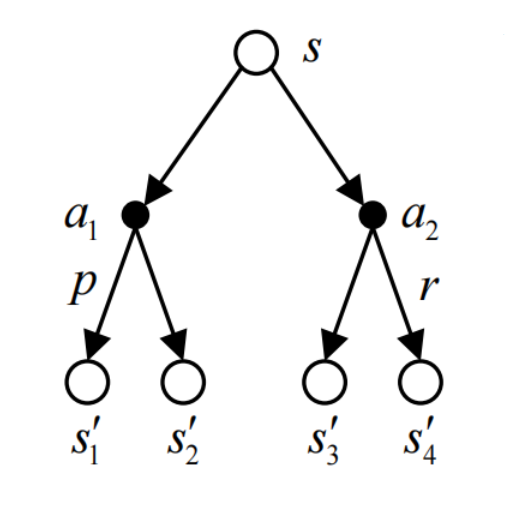
\includegraphics[width=0.3\linewidth]{images/example1_rl.png}
        \caption{例题1图}
        \label{fig:placeholder}
    \end{figure}
$${v}_{\pi }\left( s\right)  = {\mathrm{E}}_{\pi }\left( {{G}_{t} \mid  {S}_{t} = s}\right)$$
$$= \pi \left( {{a}_{1} \mid  s}\right) p\left( {{s}_{1}^{\prime },{r}_{1} \mid  s,{a}_{1}}\right) \left\lbrack  {{r}_{1} + \gamma {v}_{\pi }\left( {s}_{1}^{\prime }\right) }\right\rbrack$$
$$+ \pi \left( {{a}_{1} \mid  s}\right) p\left( {{s}_{2}^{\prime },{r}_{2} \mid  s,{a}_{1}}\right) \left\lbrack  {{r}_{2} + \gamma {v}_{\pi }\left( {s}_{2}^{\prime }\right) }\right\rbrack$$
$$+ \pi \left( {{a}_{2} \mid  s}\right) p\left( {{s}_{3}^{\prime },{r}_{3} \mid  s,{a}_{2}}\right) \left\lbrack  {{r}_{3} + \gamma {v}_{\pi }\left( {s}_{3}^{\prime }\right) }\right\rbrack$$
$$+ \pi \left( {{a}_{2} \mid  s}\right) p\left( {{s}_{4}^{\prime },{r}_{4} \mid  s,{a}_{2}}\right) \left\lbrack  {{r}_{4} + \gamma {v}_{\pi }\left( {s}_{4}^{\prime }\right) }\right\rbrack$$  
    
    
    }

    {\small\kaishu
    例题2：确定环境扫地机器人任务：在确定情况下扫地机器人任务中，采用的随机策略为
$$
\pi(a\mid S_i)=\frac{1}{|A(S_i)|},\qquad a\in A(S_i)
$$
其中，$|A(S_i)|$ 表示状态 $S_i$ 下可采取的动作个数。

现设折扣率 $\gamma=0.8$，求扫地机器人任务中各个状态的状态值函数。

\begin{itemize}
    \item 由状态值函数的贝尔曼方程，
    $$
    v_{\pi}(S_i)=\sum_{a\in A(S_i)}\pi(a\mid S_i)\sum_{s',r}p(s',r\mid S_i,a)\big[r+\gamma v_{\pi}(s')\big]
    $$
    
    \item 由于本题为确定环境，所以状态转移是确定的，即对每个动作 $a$，都会唯一对应一个下一状态 $s'$ 和即时奖赏 $r$，因此
    $$
    p(s',r\mid S_i,a)=1
    $$
    故上式可写成
    $$
    v_{\pi}(S_i)=\sum_{a\in A(S_i)}\pi(a\mid S_i)\big[r(S_i,a)+\gamma v_{\pi}(s')\big]
    $$

    \item 下面以状态 $S_1$ 为例说明各项取值的具体含义：

    在状态 $S_1$ 下，有 $3$ 个可选动作，因此
    $$
    |A(S_1)|=3,\qquad \pi(a\mid S_1)=\frac{1}{3}
    $$
    
    由图中状态转移关系可知，$S_1$ 的三个动作分别对应：
    \begin{itemize}
        \item 转移到 $S_6$，即时奖赏为 $0$；
        \item 转移到终止状态， 即时奖赏为 $1$，终止状态的状态值记为 $0$；
        \item 转移到 $S_2$，即时奖赏为 $0$。
    \end{itemize}
    
    因此
    $$
    v_{\pi}(S_1)
    =\frac{1}{3}\bigl(0+0.8\,v_{\pi}(S_6)\bigr)
    +\frac{1}{3}\bigl(1+0.8\times 0\bigr)
    +\frac{1}{3}\bigl(0+0.8\,v_{\pi}(S_2)\bigr)
    $$
    

    \item 同理，可以列出其余状态的状态值方程组。由题图可得：
    $$
    \left\{
    \begin{aligned}
    v_{\pi}(S_1)
    &=\frac{1}{3}\bigl(0+0.8\,v_{\pi}(S_6)\bigr)
     +\frac{1}{3}\bigl(1+0.8\times 0\bigr)
     +\frac{1}{3}\bigl(0+0.8\,v_{\pi}(S_2)\bigr) \\
    v_{\pi}(S_2)
    &=\frac{1}{3}\bigl(0+0.8\,v_{\pi}(S_7)\bigr)
     +\frac{1}{3}\bigl(0+0.8\,v_{\pi}(S_1)\bigr)
     +\frac{1}{3}\bigl(0+0.8\,v_{\pi}(S_3)\bigr) \\
    &\qquad \vdots \\
    v_{\pi}(S_{11})
    &=\frac{1}{4}\bigl(0+0.8\,v_{\pi}(S_{16})\bigr)
     +\frac{1}{4}\bigl(0+0.8\,v_{\pi}(S_6)\bigr)
     +\frac{1}{4}\bigl(0+0.8\,v_{\pi}(S_{10})\bigr)
     +\frac{1}{4}\bigl(-10+0.8\,v_{\pi}(S_{11})\bigr) \\
    &\qquad \vdots \\
    v_{\pi}(S_{13})
    &=\frac{1}{4}\bigl(0+0.8\,v_{\pi}(S_{18})\bigr)
     +\frac{1}{4}\bigl(0+0.8\,v_{\pi}(S_8)\bigr)
     +\frac{1}{4}\bigl(-10+0.8\,v_{\pi}(S_{13})\bigr)
     +\frac{1}{4}\bigl(0+0.8\,v_{\pi}(S_{14})\bigr) \\
    &\qquad \vdots \\
    v_{\pi}(S_{23})
    &=\frac{1}{3}\bigl(0+0.8\,v_{\pi}(S_{18})\bigr)
     +\frac{1}{3}\bigl(0+0.8\,v_{\pi}(S_{22})\bigr)
     +\frac{1}{3}\bigl(0+0.8\,v_{\pi}(S_{24})\bigr) \\
    v_{\pi}(S_{24})
    &=\frac{1}{2}\bigl(3+0.8\times 0\bigr)
     +\frac{1}{2}\bigl(0+0.8\,v_{\pi}(S_{23})\bigr)
    \end{aligned}
    \right.
    $$

    \item 由上述方程组联立求解，即可得到各状态的状态值。
\end{itemize}
}

\item \textbf{最优策略与最优值函数：}
\begin{itemize}
    \item 利用强化学习方法解决任务的关键在于：搜索出 MDP 中的最优策略。
    
    \item \textbf{最优策略：}最优策略就是使得值函数最大的策略。在有限 MDP 中，由于状态空间和动作空间都是有限的，因此策略也是有限的。
    
    \item \textbf{更优策略：}若策略 $\pi'$ 在\textbf{所有状态}下的期望回报都大于或等于策略 $\pi$ 的期望回报，则称 $\pi'$ 优于 $\pi$，记为 $\pi'\geq \pi$。即对于所有 $s\in S$，都有
    $$
    v_{\pi'}(s)\geq v_{\pi}(s)
    $$
    
    \item \textbf{最优状态值函数：}最优策略可能不止一个，但它们共享相同的状态值函数，定义为
    $$
    v_{*}(s)=v_{\pi_*}(s)=\max_{\pi}v_{\pi}(s),\qquad s\in S
    $$
    
    \item \textbf{最优动作值函数：}在状态 $s$ 处执行动作 $a$，并在随后过程中采取最优策略 $\pi_*$ 所得到的期望回报，定义为
    $$
    q_{*}(s,a)=q_{\pi_*}(s,a)=\max_{\pi}q_{\pi}(s,a),\qquad s\in S,\ a\in A
    $$
\end{itemize}
\item \textbf{贝尔曼最优方程：}
\begin{itemize}
    \item \textbf{基于状态值的贝尔曼最优方程：}
    
    由最优状态值函数的定义可得
    $$
    v_{*}(s)=\max_{a\in A(s)}q_{\pi_*}(s,a)
    $$
    
    又因为
    $$
    q_{\pi_*}(s,a)=\mathbb{E}_{\pi_*}(R_{t+1}+\gamma G_{t+1}\mid S_t=s,A_t=a)
    $$
    
    从而有
    $$
    \begin{aligned}
    v_{*}(s)
    &=\max_{a} \mathbb{E}_{\pi_*}(R_{t+1}+\gamma G_{t+1}\mid S_t=s,A_t=a)\\
    &=\max_{a} \mathbb{E}(R_{t+1}+\gamma v_{*}(S_{t+1})\mid S_t=s,A_t=a)\\
    &=\max_{a}\sum_{s',r}p(s',r\mid s,a)\big[r+\gamma v_{*}(s')\big]
    \end{aligned}
    $$
    
    \item \textbf{基于动作值的贝尔曼最优方程：}
    
    类似地，可以得到最优动作值函数满足
    $$
    \begin{aligned}
    q_{*}(s,a)
    &=\mathbb{E}(R_{t+1}+\gamma v_{*}(S_{t+1})\mid S_t=s,A_t=a)\\
    &=\mathbb{E}\!\left(R_{t+1}+\gamma \max_{a'}q_{*}(S_{t+1},a')\mid S_t=s,A_t=a\right)\\
    &=\sum_{s',r}p(s',r\mid s,a)\left[r+\gamma \max_{a'}q_{*}(s',a')\right]
    \end{aligned}
    $$
\end{itemize}
\begin{figure}
    \centering
    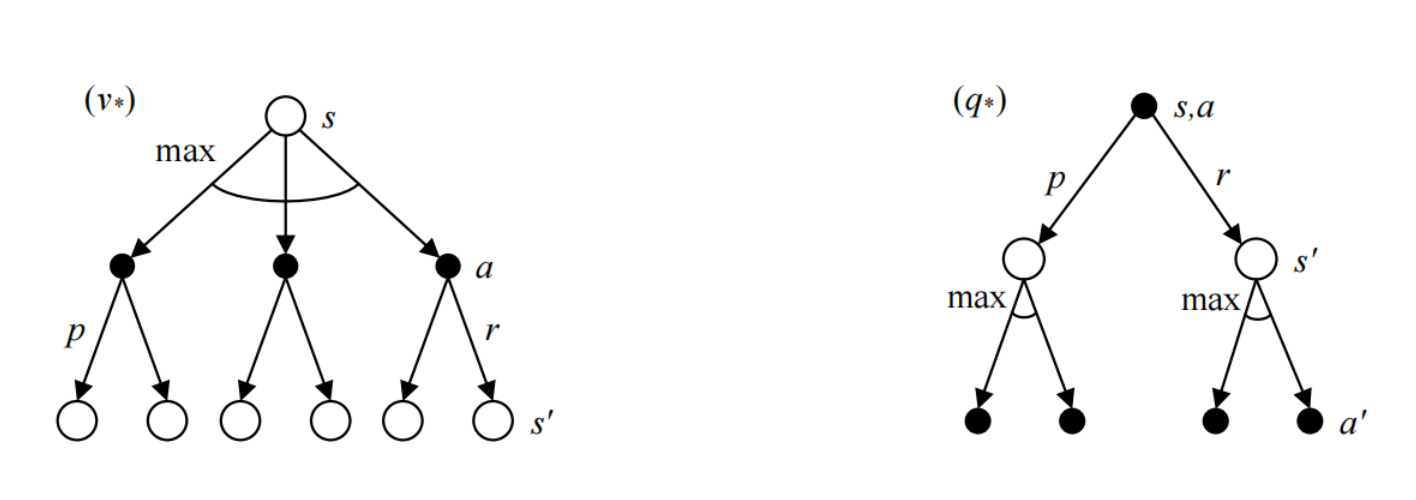
\includegraphics[width=0.5\linewidth]{images/fangcheng.png}
    \caption{对比：基于状态值（左）/动作值（右）的贝尔曼最优方程更新图}
    \label{fig:placeholder}
\end{figure}
    \end{itemize}

    \item \textbf{强化学习的一大矛盾：}探索与利用的平衡\footnote{利用就是为了最大回报要始终采用最优动作，根据当前的值函数最大限度提升回报；探索就是摒弃基于值函数的贪心策略，找到更多可能的动作来获得更好的策略，探索更多的可能性。}
\end{enumerate}










\end{document}
